\documentclass[a4paper,11.5pt]{article}
\usepackage[textwidth=170mm, textheight=230mm, inner=20mm, top=20mm, bottom=30mm]{geometry}
\usepackage[normalem]{ulem}
\usepackage[utf8]{inputenc}
\usepackage[T1]{fontenc}
\PassOptionsToPackage{defaults=hu-min}{magyar.ldf}
\usepackage{pgfplots}
\pgfplotsset{compat=1.10}
\usepgfplotslibrary{fillbetween}
\usepackage[magyar]{babel}
\usepackage{amsmath, amsthm,amssymb,paralist,array, ellipsis, graphicx, float, bigints,tikz}
%\usepackage{marvosym}

\makeatletter
\renewcommand*{\mathellipsis}{%
	\mathinner{%
		\kern\ellipsisbeforegap%
		{\ldotp}\kern\ellipsisgap
		{\ldotp}\kern\ellipsisgap%
		{\ldotp}\kern\ellipsisaftergap%
	}%
}
\renewcommand*{\dotsb@}{%
	\mathinner{%
		\kern\ellipsisbeforegap%
		{\cdotp}\kern\ellipsisgap%
		{\cdotp}\kern\ellipsisgap%
		{\cdotp}\kern\ellipsisaftergap%
	}%
}
\renewcommand*{\@cdots}{%
	\mathinner{%
		\kern\ellipsisbeforegap%
		{\cdotp}\kern\ellipsisgap%
		{\cdotp}\kern\ellipsisgap%
		{\cdotp}\kern\ellipsisaftergap%
	}%
}
\renewcommand*{\ellipsis@default}{%
	\ellipsis@before
	\kern\ellipsisbeforegap
	.\kern\ellipsisgap
	.\kern\ellipsisgap
	.\kern\ellipsisgap
	\ellipsis@after\relax}
\renewcommand*{\ellipsis@centered}{%
	\ellipsis@before
	\kern\ellipsisbeforegap
	.\kern\ellipsisgap
	.\kern\ellipsisgap
	.\kern\ellipsisaftergap
	\ellipsis@after\relax}
\AtBeginDocument{%
	\DeclareRobustCommand*{\dots}{%
		\ifmmode\@xp\mdots@\else\@xp\textellipsis\fi}}
\def\ellipsisgap{.1em}
\def\ellipsisbeforegap{.05em}
\def\ellipsisaftergap{.05em}
\makeatother

\usepackage{hyperref}
\hypersetup{
	colorlinks = true	
}

\DeclareMathOperator{\Int}{int}
\DeclareMathOperator{\tg}{tg}
\DeclareMathOperator{\ctg}{ctg}
\DeclareMathOperator{\Th}{th}
\DeclareMathOperator{\sh}{sh}
\DeclareMathOperator{\ch}{ch}
\DeclareMathOperator{\arsh}{arsh}
\DeclareMathOperator{\arch}{arch}
\DeclareMathOperator{\arth}{arth}
\DeclareMathOperator{\arcth}{arcth}
\DeclareMathOperator{\grad}{grad}
\DeclareMathOperator{\arc}{arc}
\DeclareMathOperator{\arctg}{arc tg}
\DeclareMathOperator{\arcctg}{arc ctg}
\newcommand{\norm}[1]{\left\lVert#1\right\rVert}

\begin{document}
	%%%%%%%%%%%RÖVIDÍTÉSEK%%%%%%%%%%
	\setlength\parindent{0pt}
	\def\a{\textbf{a}}
	\def\b{\textbf{b}}
	\def\N{\hskip 10 true mm}
	\def\a{\textbf{a}}
	\def\b{\textbf{b}}
	\def\c{\textbf{c}}
	\def\d{\textbf{d}}
	\def\e{\textbf{e}}
	\def\gg{$\gamma$}
	\def\vi{\textbf{i}}
	\def\jj{\textbf{j}}
	\def\kk{\textbf{k}}
	\def\fh{\overrightarrow}
	\def\l{\lambda}
	\def\m{\mu}
	\def\v{\textbf{v}}
	\def\0{\textbf{0}}
	\def\s{\hspace{0.2mm}\vphantom{\beta}}
	\def\Z{\mathbb{Z}}
	\def\Q{\mathbb{Q}}
	\def\R{\mathbb{R}}
	\def\C{\mathbb{C}}
	\def\N{\mathbb{N}}
	\def\Rn{\mathbb{R}^{n}}
	\def\Ra{\overline{\mathbb{R}}}
	\def\sume{\displaystyle\sum_{n=1}^{+\infty}}
	\def\sumn{\displaystyle\sum_{n=0}^{+\infty}}
	\def\biz{\emph{Bizonyítás:\ }}
	\def\narrow{\underset{n\rightarrow+\infty}{\longrightarrow}}
	\def\limn{\displaystyle\lim_{n\to +\infty}}
	%	\def\definition{\textbf{Definíció:\ }}
	%	\def\theorem{\textbf{Tétel:\ }}
	%\def\note{\emph{Megjegyzés:\ }}
	%\def\example{\textbf{Példa:\ }} 
	
	\theoremstyle{definition}
	\newtheorem{theorem}{Tétel}[subsubsection] % reset theorem numbering for each chapter
	
	\theoremstyle{definition}
	\newtheorem{definition}[theorem]{Definíció} % definition numbers are dependent on theorem numbers
	\newtheorem{example}[theorem]{Példa} % same for example numbers
	\newtheorem{exercise}[theorem]{Házi feladat} % same for example numbers
	\newtheorem{note}[theorem]{Megjegyzés} % same for example numbers
	\newtheorem{task}[theorem]{Feladat} % same for example numbers
	\newtheorem{revision}[theorem]{Emlékeztető} % same for example numbers
	%%%%%%%%%%%%%%%%%%%%%%%%%%%%%%%%%
	\begin{center}
		{\LARGE\textbf{Analízis 3. A szakirány}}
		\smallskip
		
		{\Large Gyakorlati jegyzet}
		
		\smallskip
		8. óra.
	\end{center}
	A jegyzetet \textsc{Umann} Kristóf készítette \textsc{Filipp} Zoltán István gyakorlatán. (\today)
	\subsection{Folytonosság}
	\begin{example}
		\[ f(x,y):=\begin{cases}
			\frac{xy}{x^2+y^2},\quad (x,y)\in\R^2\setminus\{ (0,0) \}\\
			0,\quad (x,y)=(0,0)
		\end{cases} \]
		Vizsgáljuk az $f$ folytonosságát!
		
		\textit{Megoldás:}
		\begin{enumerate}
			\item $\forall y_0\in\R\quad \Rightarrow\quad g(x):=f(x,y_0) \quad (x\in\R,\quad g\in C(\R))$
			\item $\forall x_0\in\R\quad \Rightarrow\quad h(y):=f(x_0,y)\quad (y\in\R,\quad  h\in C(\R))$
			\item $f\notin C\{(0,0)\}$
		\end{enumerate}
		\begin{figure}[H]
			\centering
			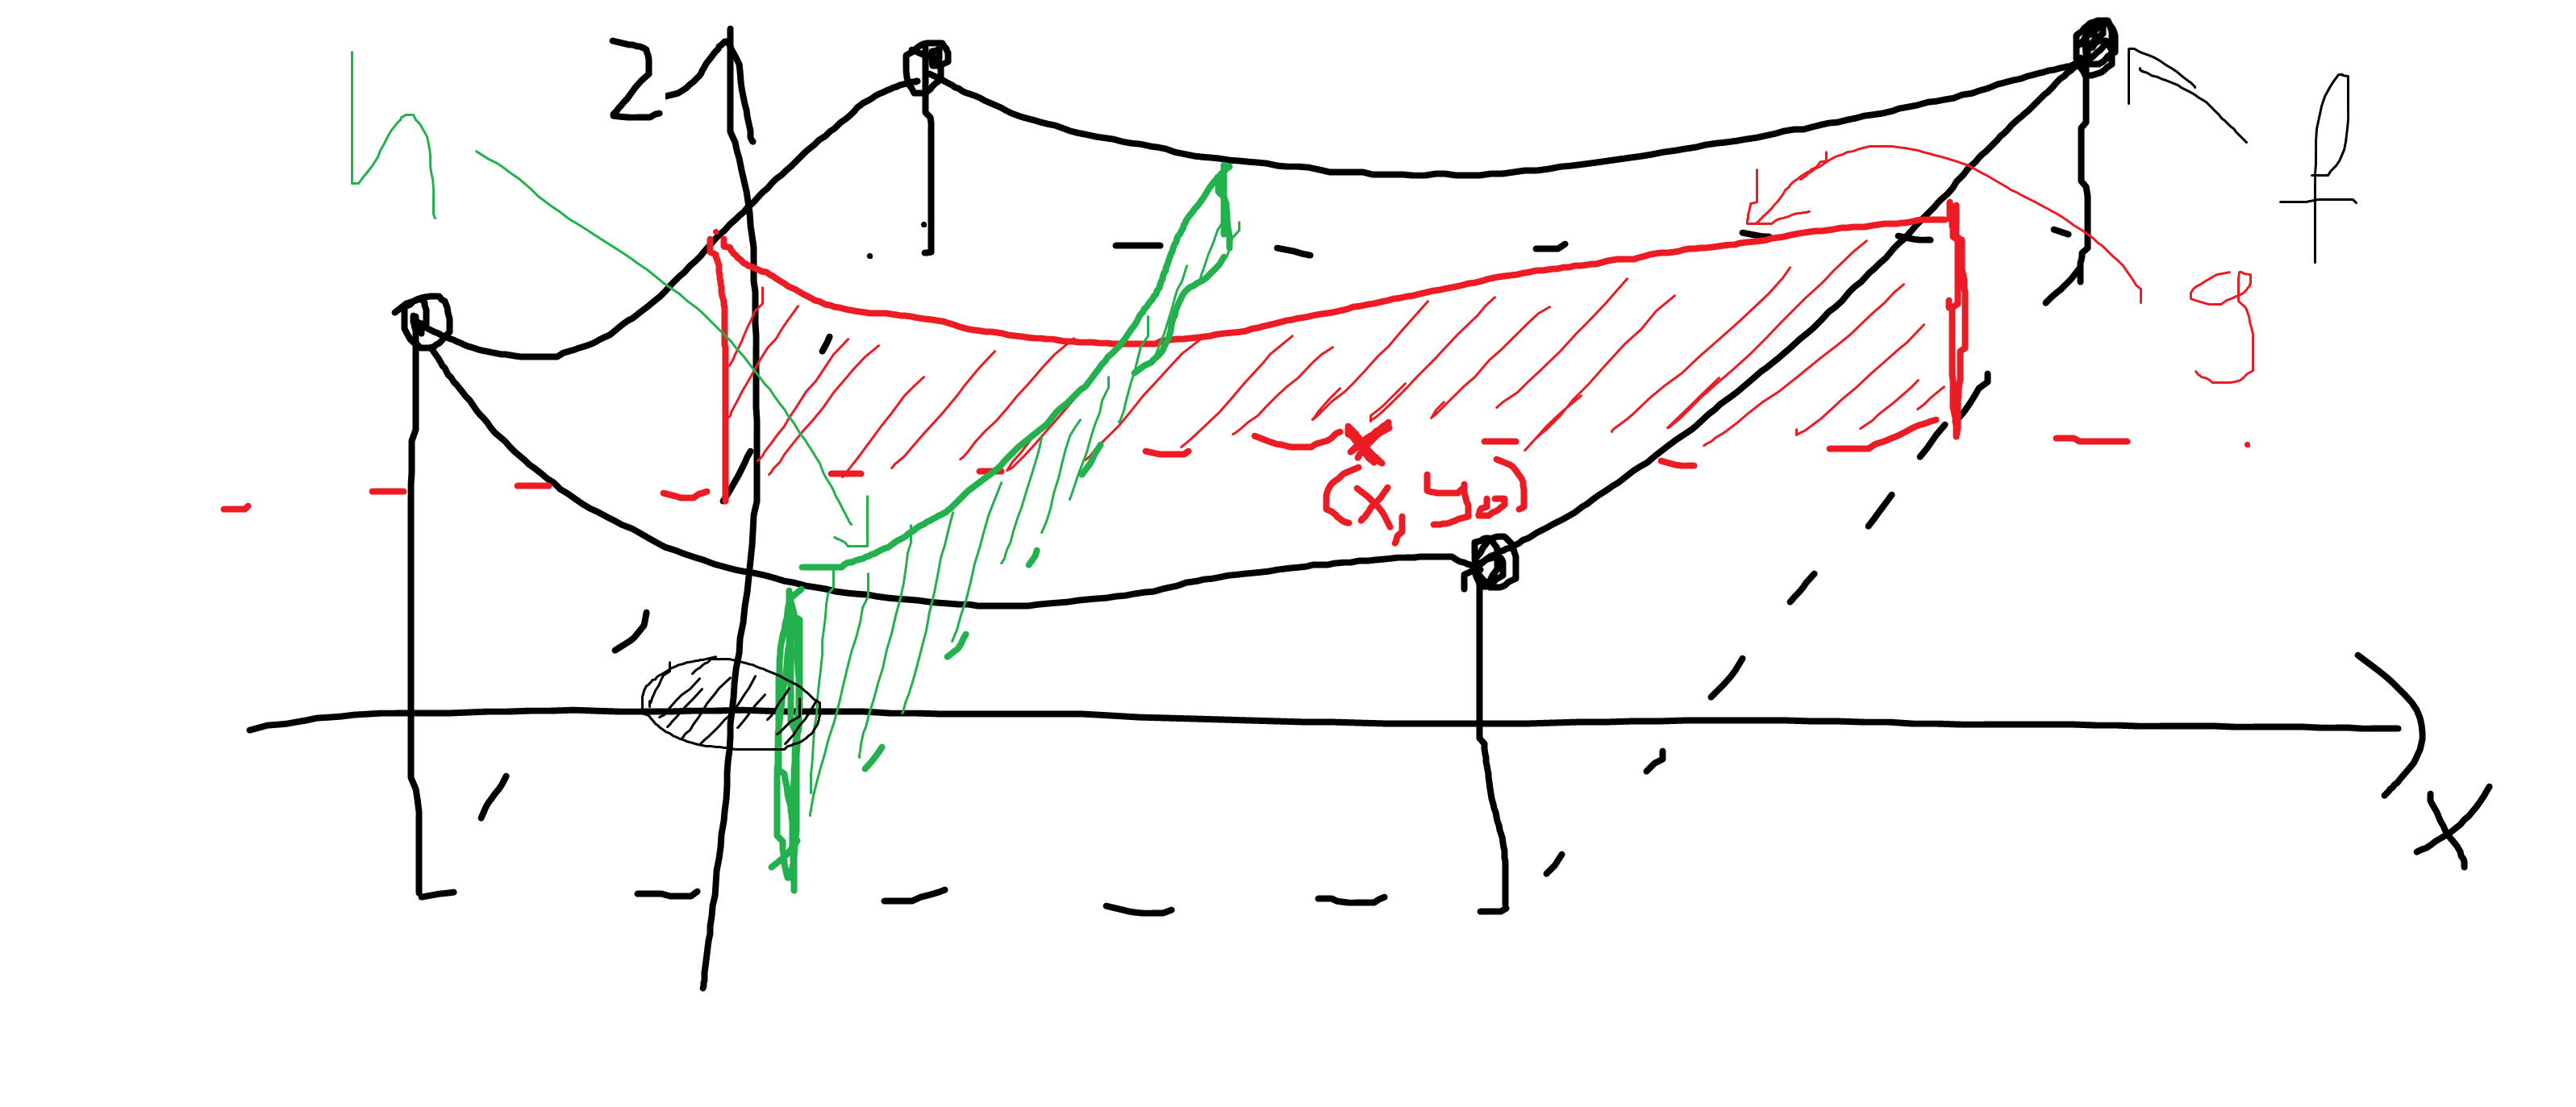
\includegraphics[height=3cm]{../2zh/kepek/25.png}
			\caption{}
		\end{figure}
		\textit{Bizonyítás:}
		
		\begin{enumerate}
			\item Ha $y_0=0$:
			\[ g(x)=\begin{cases}
				\frac{x\cdot0}{x^2+0^2}=\frac{0}{x^2}=0\quad x\not=0\\
				0,\quad (x,0)=(0,0)\quad \Leftrightarrow\quad x=0
			\end{cases} \]
			\[ \Rightarrow\quad g(x)=0\quad (\forall x\in\R) \quad \Rightarrow\quad g\in C(\R) \]
			Ha $y_0\in\R\setminus\{ 0 \}$:
			\[ g(x)=f(x,y_0)=\begin{cases}
			\frac{xy_0}{ x^2+y_0^2 }\quad x\in\R\\
			\text{(nem lehetséges)}
			\end{cases}\]
			$\Rightarrow\quad g(x)=\frac{xy_0}{x^2+\underbrace{y_0^2}_{\not=0}}\quad (x\in\R)$ és ez folytonos (ld. racionális törtfüggvények)
			\item Ennek a megállapításra a másik komponensre házi feladat, azonban könnyű látni hogy nagyon hasonló lesz az eredmény, $h$ függvény is folytonos lesz.
			\item Vizsgáljuk a (0,0) pontban a határértéket, több irányból!
			\[ f(0,0)=0\quad \overset{?}{=}\ \lim_{(x,y)\to(0,0)}\frac{xy}{x^2+y^2} \]
			\[ y=0\quad \text{mentén}\quad \Rightarrow\quad \lim_{x\to0}\left(\frac{x\cdot0}{x^2+0^2}\right)=\lim_{x\to0}\frac{0}{x^2}=\lim_{x\to0}(0)=0 \]
			Ez alapján ha $\exists\lim$, akkor az csak 0 lehet. De:
			\[ y=x\quad \text{mentén}\quad \lim_{(x,x)\to(0,0)}\frac{x^2}{2x^2}\quad\overset{x\not=0}{=} \quad \lim_{x\to0}\frac{1}{2}=\frac{1}{2} \]
			Ezzel ellentmondásra jutottunk, $\Rightarrow\nexists\lim_{(0,0)}f\Rightarrow\quad f\notin C\{ (0,0) \}$ 
		\end{enumerate}
	\end{example}
	\begin{task}
		Vegyünk egy olyan függvényt, mely az origón $y$ tengely körül metszve folytonos, de 0-ban mégsem!
		\[ f(x,y):=\begin{cases}
			\frac{x^2y}{x^4+y^2}\quad (x,y)\not=(0,0)\\
			0,\quad (x,y)=(0,0)
		\end{cases} \]
		\begin{enumerate}
			\item $\forall$ origón átmenő $l:=mx$ egyenes ,,mentén'' $f$ folytonos ($f|_l\in C$)
			\item $f\notin C\{ (0,0) \}$
		\end{enumerate}
		\textit{Megoldás:}
		\begin{figure}[H]
			\centering
			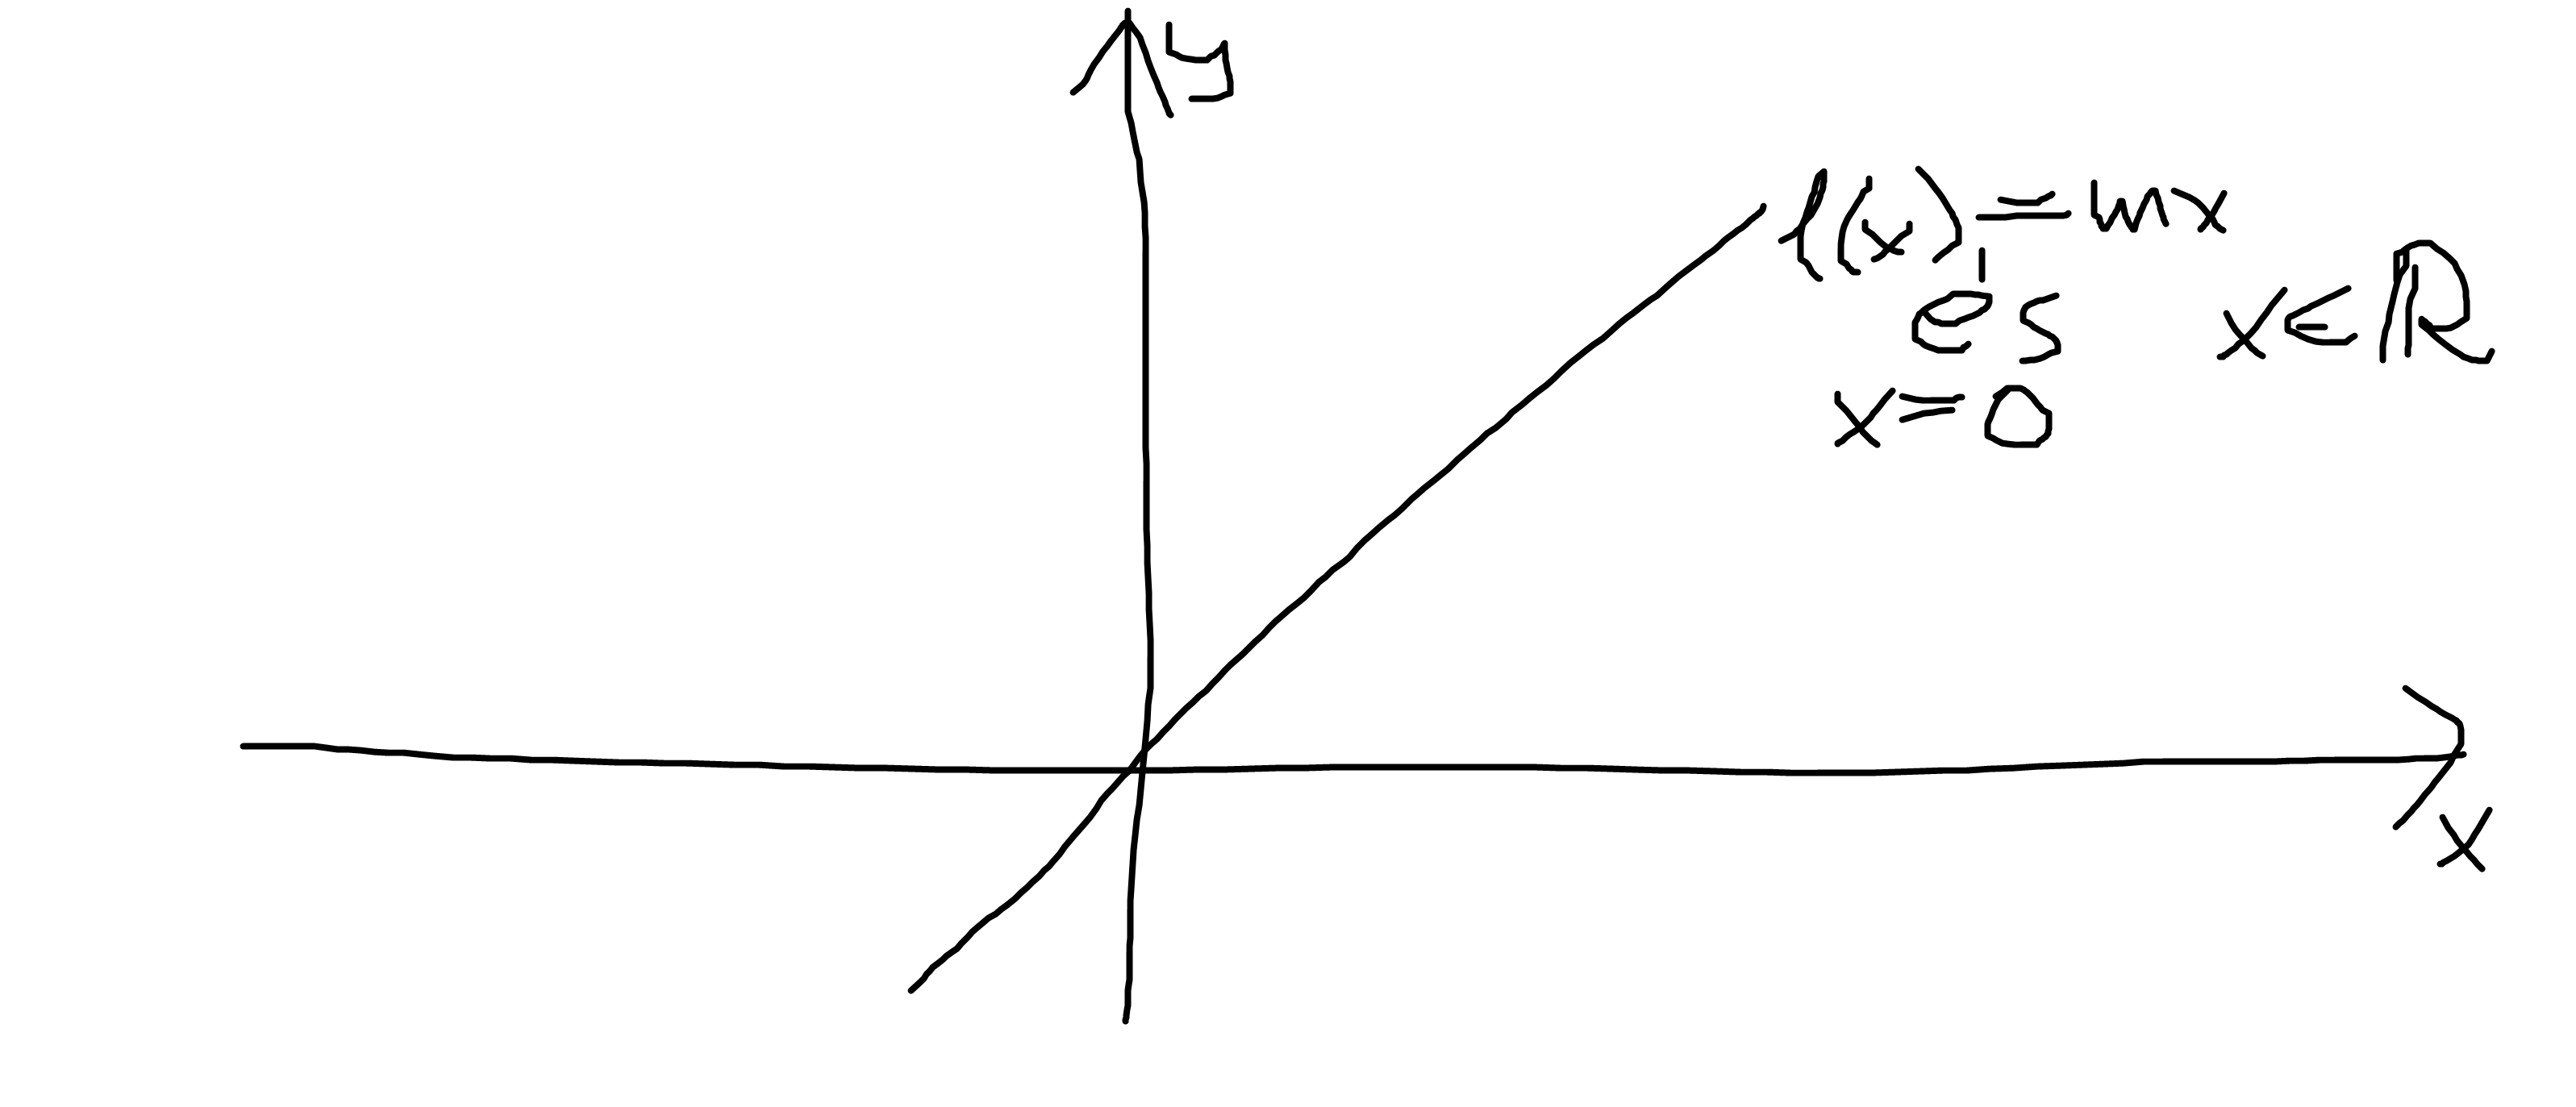
\includegraphics[height=3cm]{../2zh/kepek/26.png}
			\caption{Megjegyzendő, hogy $x=0$ nem függvény.}
		\end{figure}
		\begin{enumerate}
			\item\begin{enumerate}
				\item Ha \fbox{$x=0$}:
				\[ h(y):=f(0,y)=\begin{cases}
					\frac{0}{y^2}\quad \text{ha}\quad y\not=0\\
					0\quad y=0
				\end{cases}=0\] 
				Így $h\in C(\R)$.
				\item Ha \fbox{$m=0$}$\quad \Rightarrow\quad l(x)=0$\quad ($x$-tengely)
				\[ g(x):=f(x,0)=\begin{cases}
					\frac{0}{x^4}\quad x\not=0\\
					0,\quad x=0
				\end{cases}=0\quad\Rightarrow\quad  g\equiv0\]
				Így $g\in C(\R)$.
				\item Ha \fbox{$y=mx$}$\quad (m\in\R\setminus\{0\}):$
				\[ g(x):=f(x,mx)=\begin{cases}
					\frac{x^2mx}{x^4+m^2x^2},\quad \text{ha}\quad (x,mx)\not=(0,0)\\
					0\quad \text{ha}\quad (x,\underbrace{m}_{\not=0}x)=(0,0)
				\end{cases}\quad  \Rightarrow\quad g(x)=\begin{cases}
					\frac{mx}{x^2+m^2}\quad x\not=0\\
					0\quad x=0
				\end{cases} \]
				$g\in C(\R\setminus\{0\})$\quad (rac. törtfüggvények, nevező $\not=0$). $0$ pontban is belátható a folytonosság:
				\[ g(0)=0\overset{?}{=}\lim_{x\to0}\left(\frac{mx}{x^2+m^2}\right)=\frac{0}{\underbrace{m^2}_{\not=0}}=0 \]
				$g\in C\{0\}$ is.
			\end{enumerate}
			\item $f\notin C\{ (0,0) \}$\quad ui.:
			\[ f(0,0)=0\overset{?}{=}\lim_{(x,y)\to(0,0)}\left(\frac{x^2y}{x^4+y^2}\right) \]
			Próbáljuk a 0 pontot olyan irányokból közelíteni, hogy ellentmondásra jussunk!
			
			Ha $\displaystyle y=0\quad \Rightarrow\lim_{x\to0}\frac{0}{\underbrace{x^4}_{\not=0}}=\lim_{x\to0}(0)=0$
			
			Ha $\displaystyle y=x\quad \Rightarrow\quad \lim_{x\to0}\left(\frac{x^3}{x^4+x^2}\right)=\lim\left(\frac{x}{x^2+1}\right)=\frac{0}{1}=0$
			
			\begin{figure}[H]
				\centering
				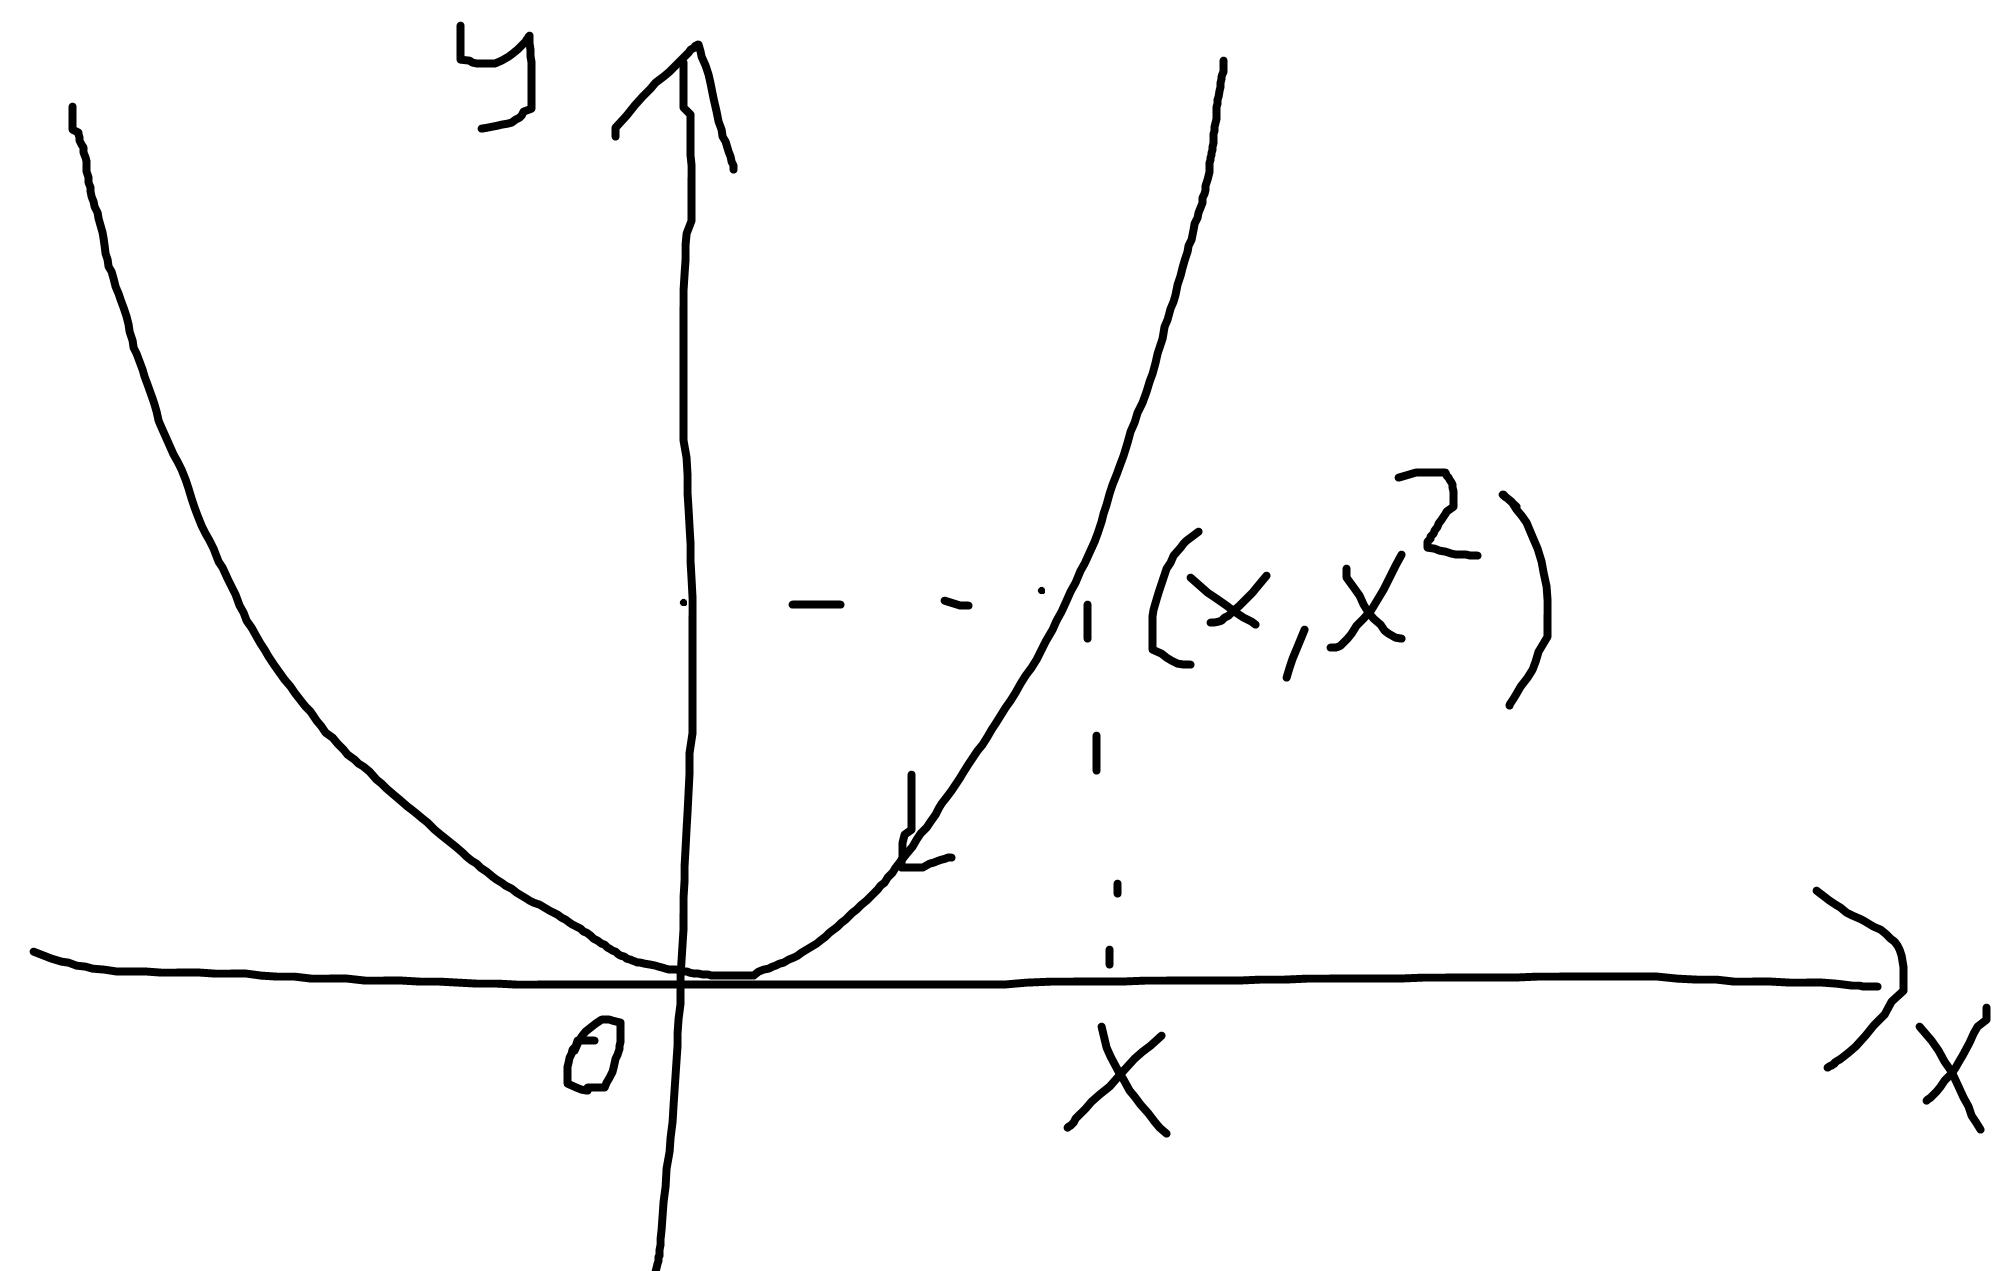
\includegraphics[height=3cm]{../2zh/kepek/27.png}
				\caption{}
			\end{figure}
			Ha $\displaystyle y = x^2\quad \Rightarrow\quad \lim_{x\to0}\frac{x^2\cdot x^2}{x^4+x^4}=\lim_{x\to0}\frac{x^4}{2x^4}=\lim_{x\to0}\frac{1}{2}=\frac{1}{2}\not=0$
			
			Így viszont már ellentmondásra jutottunk: $\nexists\lim_{(0,0)}\quad \Rightarrow \quad f\notin C\{(0,0)\}$
		\end{enumerate}
		\begin{note}
			A $g\equiv0$ azt jelenti, hogy $g$ az azonosan 0 függvény.
		\end{note}
	\end{task}
	\subsection{Differenciálás}
	\begin{task} 
		Mutassok meg hogy erősen deriválható $f$ az $a:=(1,2)$ pontban.
		\[ f(x,y):=2x^2+3xy-y^2 \quad ((x,y)\in\R^2) \]
		$\Rightarrow\quad f\in D\{a\}\quad \text{és}\quad f'(1,2)=?\quad \text{és}$ ellenőrzés a parciálisokkal.
		
		\textit{Megoldás:}
		\begin{revision}
			$1\leq n,m\in\N\quad f\in\R^n\to\R^m,\quad a\in \Int \mathcal{D}_f,\quad f\in D\{ a \}\quad \Leftrightarrow \quad \exists L\in\LARGE(\R^n,\R^m)$.
			\[ \lim_{h\to0} \frac{\norm{f(a+hh)-f(a)-L(h)}_{\R^m}}{\norm{h}_{\R^n}}=0 \]
		\end{revision}
		\begin{revision}
			$L\in L(\R^n,\R^m)\quad \Leftrightarrow\quad \exists A\in\R^{m\times n}\quad L(h)=Ah\quad (\forall h\in\R^n)$
		 Ekkor: $f'(a)=A$ Jacobi mátrix.
		\end{revision}
		\textit{Visszatérve a feladathoz:} $f:\R^2\to\R\quad \Rightarrow\quad f'(1,2)\in\R^{1\times 2}\equiv \R{^2}$.\quad 
		Legyen: $h:=(x,y),\quad a=(1,2)$
		\[ f(a+h)-f(a)=f(x+1,y+2)-f(1,2)=2(x+1)^2+3(x+1)(y+2)-(y+2)^2-4=\]\[=2x^2+4x+2+3xy+6x+3y+6-y^2-4y-4-4=\underbrace{10x-y}_{\text{lineáris tagok}}+(\underbrace{2x^2+3xy-y^2}_{\text{maradék}}) \]
		\begin{figure}[H]
			\centering
			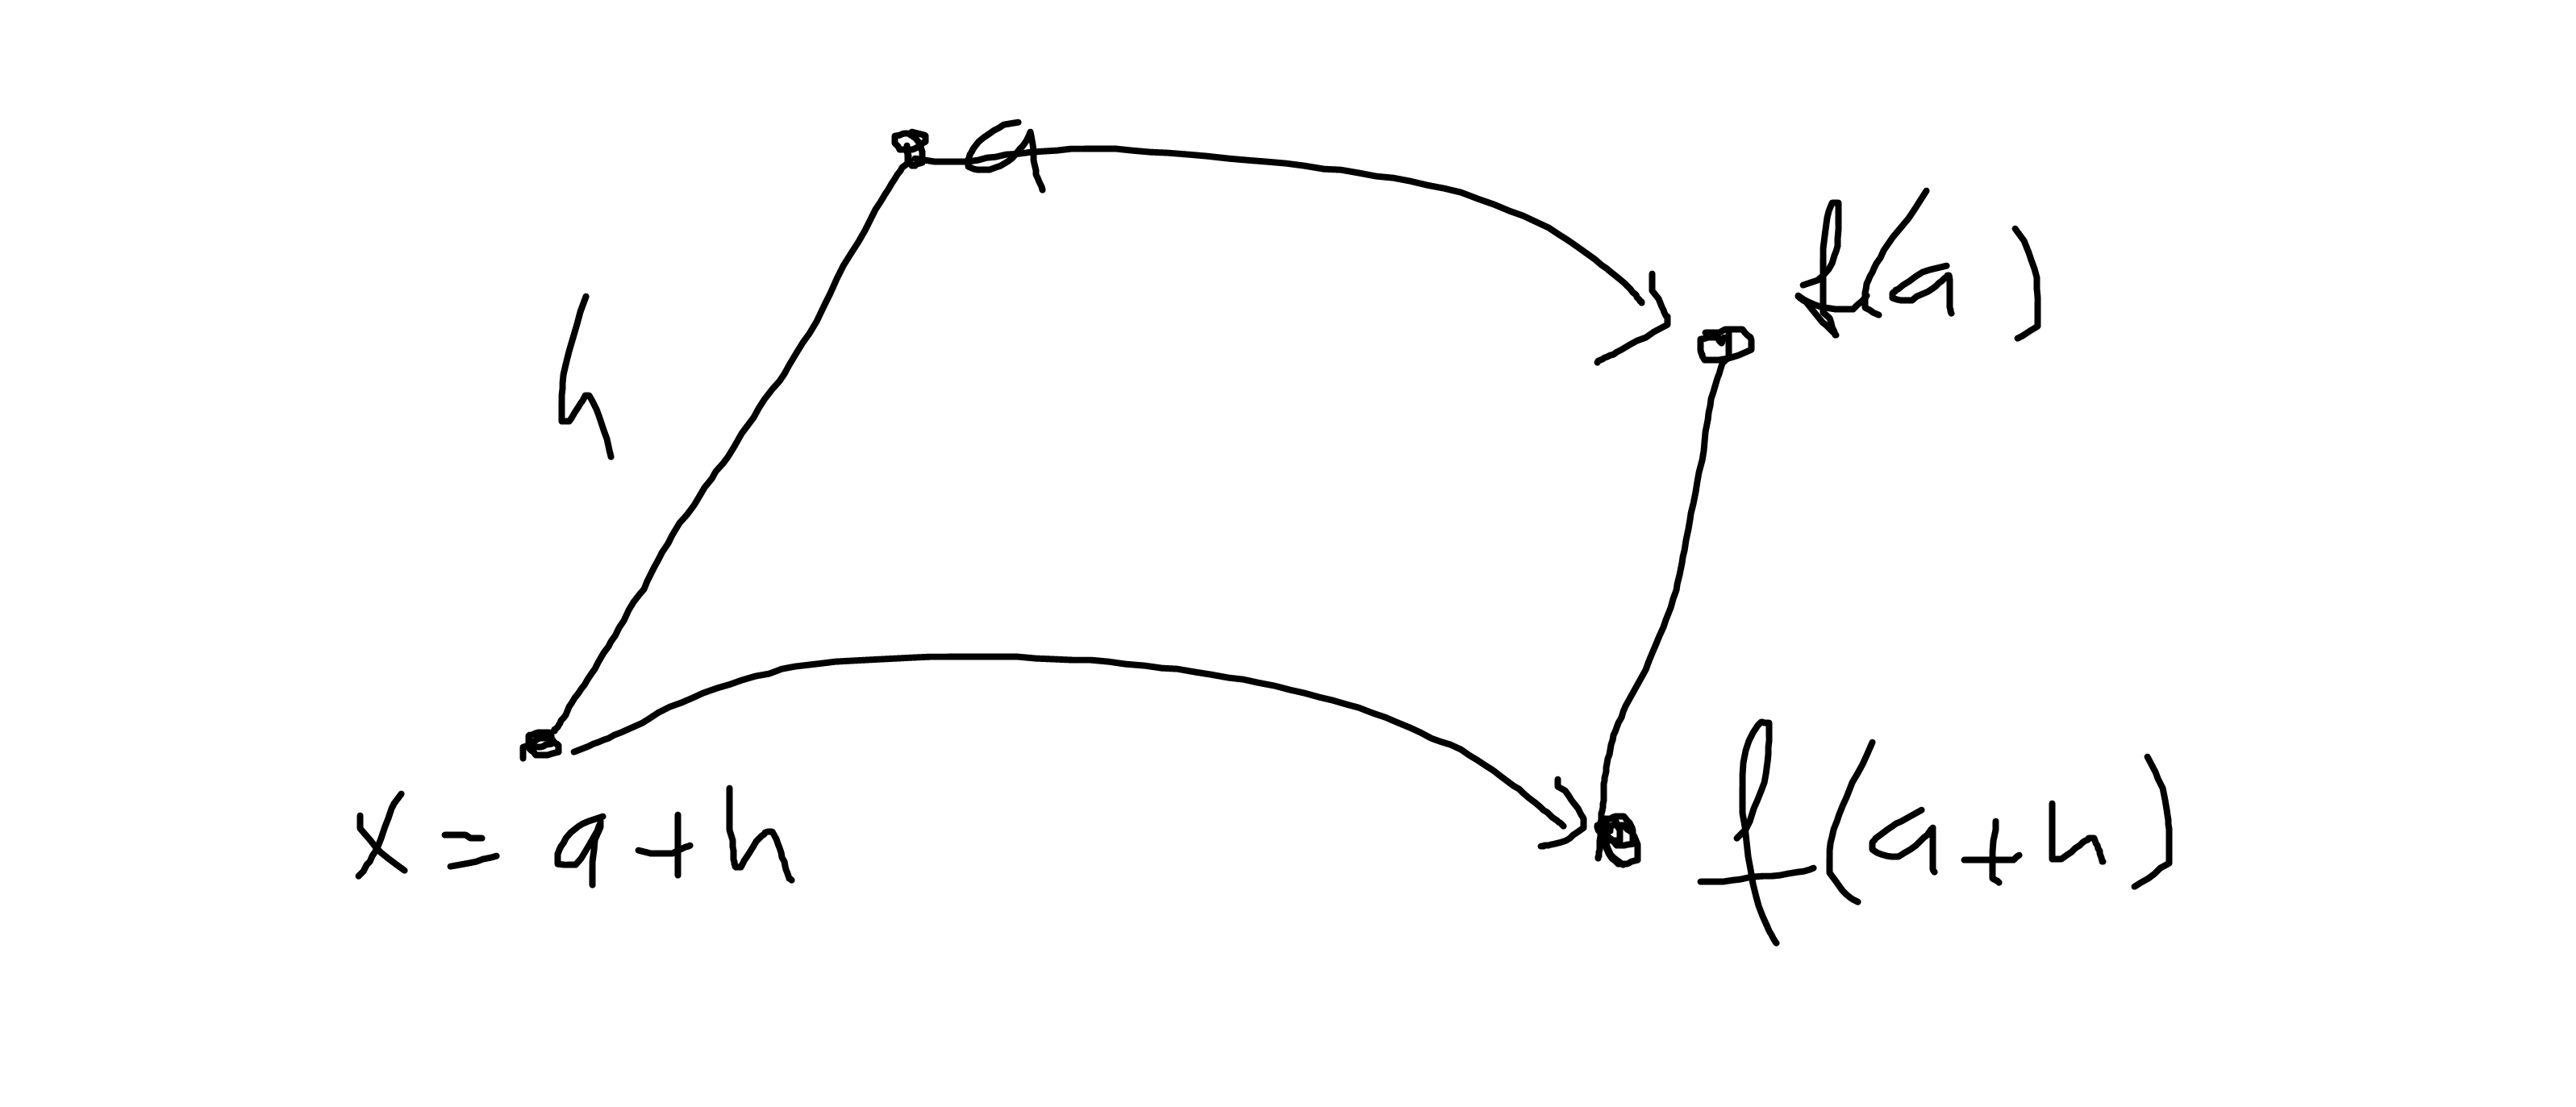
\includegraphics[height=3cm]{../2zh/kepek/28.png}
			\caption{Az analízis egyik fő gondolatmenete, hogy ha az $a$ pontot $h$-val eltoljuk, akkor ezen ponton képe hogyan változik.}
		\end{figure}
		Legyen: $L(h):=L(x,y):=10x-y=\langle(10,-1),(x,y)\rangle=\begin{bmatrix}
			10&-1
		\end{bmatrix}\cdot \begin{bmatrix}
			x\\y
		\end{bmatrix} =Ah$ ahol $A=\begin{bmatrix}
		10&-1
		\end{bmatrix}\in\R^{1\times2}$
		
		A maradéktagokkal így:
		\[ \lim_{(x,y)\to(0,0)}\frac{\overbrace{|2x^2+3xy-y^2|}^{\norm{.}_{\R^1}}}{\norm{(x,y)}_{\R^2}}\leq \]
		Tökmindegy, milyen normával dolgozunk. Itt célszerű (mint az esetek többségében is) végtelen normával dolgozni.
		\[ \overset{\text{háromszög}}{\underset{\text{egyenlőtelenség}}{\leq}}\lim_{(x,y)\to(0,0)}\frac{2|x|^2+3|x|\cdot|y|+|y|^2}{\norm{(x,y)}_\infty}\quad \overset{|x|,|y|\leq\norm{(x,y)}_\infty=}{\underset{=\max\{|x|,|y|\}}{\leq}}\quad \lim_{(x,y)\to(0,0)}\frac{6\cdot\norm{(x,y)^2}_\infty}{\norm{(x,y)}_\infty}=6\cdot0=0 \]
		Mivel normák hányadosa nemnegatív, így alsó becslésünk is van, kapásból odaírhatjuk a legelső $\lim$ elé, hogy $0\leq$ (melyet itt a csattanó kedvéért nem tettünk meg).
		\[ 0\leq\lim_{(x,y)\to(0,0)}\frac{\overbrace{|2x^2+3xy-y^2|}^{\norm{.}_{\R^1}}}{\norm{(x,y)}_{\R^2}}\leq 0\quad  \overset{\text{közrefogás}}{\Rightarrow}\quad \text{a definícióbeli $\lim$ valóban } 0. \]
		$\Rightarrow \quad f\in D\{(1,2)\}$ és $f'(1,2)=\begin{bmatrix}
		10&-1
		\end{bmatrix}$.
		\begin{note}
			Értelemszerűen, a gömbölyű és szögletes zárójel között érdemi különbség nincs, Filipp tanár úr inkább gömbölyű zárójelet használ, míg én a szögleteset szeretem jobban.
		\end{note}
		
		\textit{Ellenőrzés:}
		\begin{revision}
			Ha $f\in\R^n\to\R$ típus\quad $(m=1)$\quad és\quad $f\in D\{a\}\quad \Rightarrow$
			\[ f'(a)=\grad f(a)=(
				\partial_1 f(a), \partial_2 f(a), \dots, \partial_nf(a)) \]
		\end{revision}
		\textit{Visszatérvén az ellenőrzéshez}: $((x,y)\in\R^2)$
		\[ \partial_1 f(\overbrace{x}^{\text{változó}},\overbrace{y}^{\text{konstans}})=4x+3y \]
		\[ \partial_2f(\underbrace{x}_{\text{konstans}},\underbrace{y}_{\text{változó}})=3x-2y  \]
		$\Rightarrow\quad \exists\partial_1 f,\partial_2 f:\quad \R^2\to\R$ parciális derivált fvek és folytonosak $\R^2$-en polinomok $\overset{\text{tétel}}{\Rightarrow}\quad f\in D(\R^2)$ és 
		\[ f'(x,y)=\grad f(x,y)=(\partial_1 f(x,y),\  \partial_2f(x,y)) \]
		Ez az általunk definiált $f$ függvénnyel:
		\[ f'(x,y)=(4x+3y,3x-2y)\quad (\forall(x,y)\in\R^2) \]
		Speciálisan:
		\[ f'(1,2)=(4\cdot1+\cdot2;\ 3\cdot1-2\cdot2)=(10;\ -1) \]
	\end{task}
	\begin{note}
		Itt $\equiv$ izomorfiát jelöl.
	\end{note}
	
	\begin{task}
		\[ f(x,y)=\begin{bmatrix}
			x^3+xy\\
			x-y^2\\
			1+y
		\end{bmatrix}\quad (x,y)\in\R^2 \]
		$\exists f'(1,2)=?$ Ellenőrizzünk jacobival.
		
		\textit{Megoldás:}
		\begin{figure}[H]
			\centering
			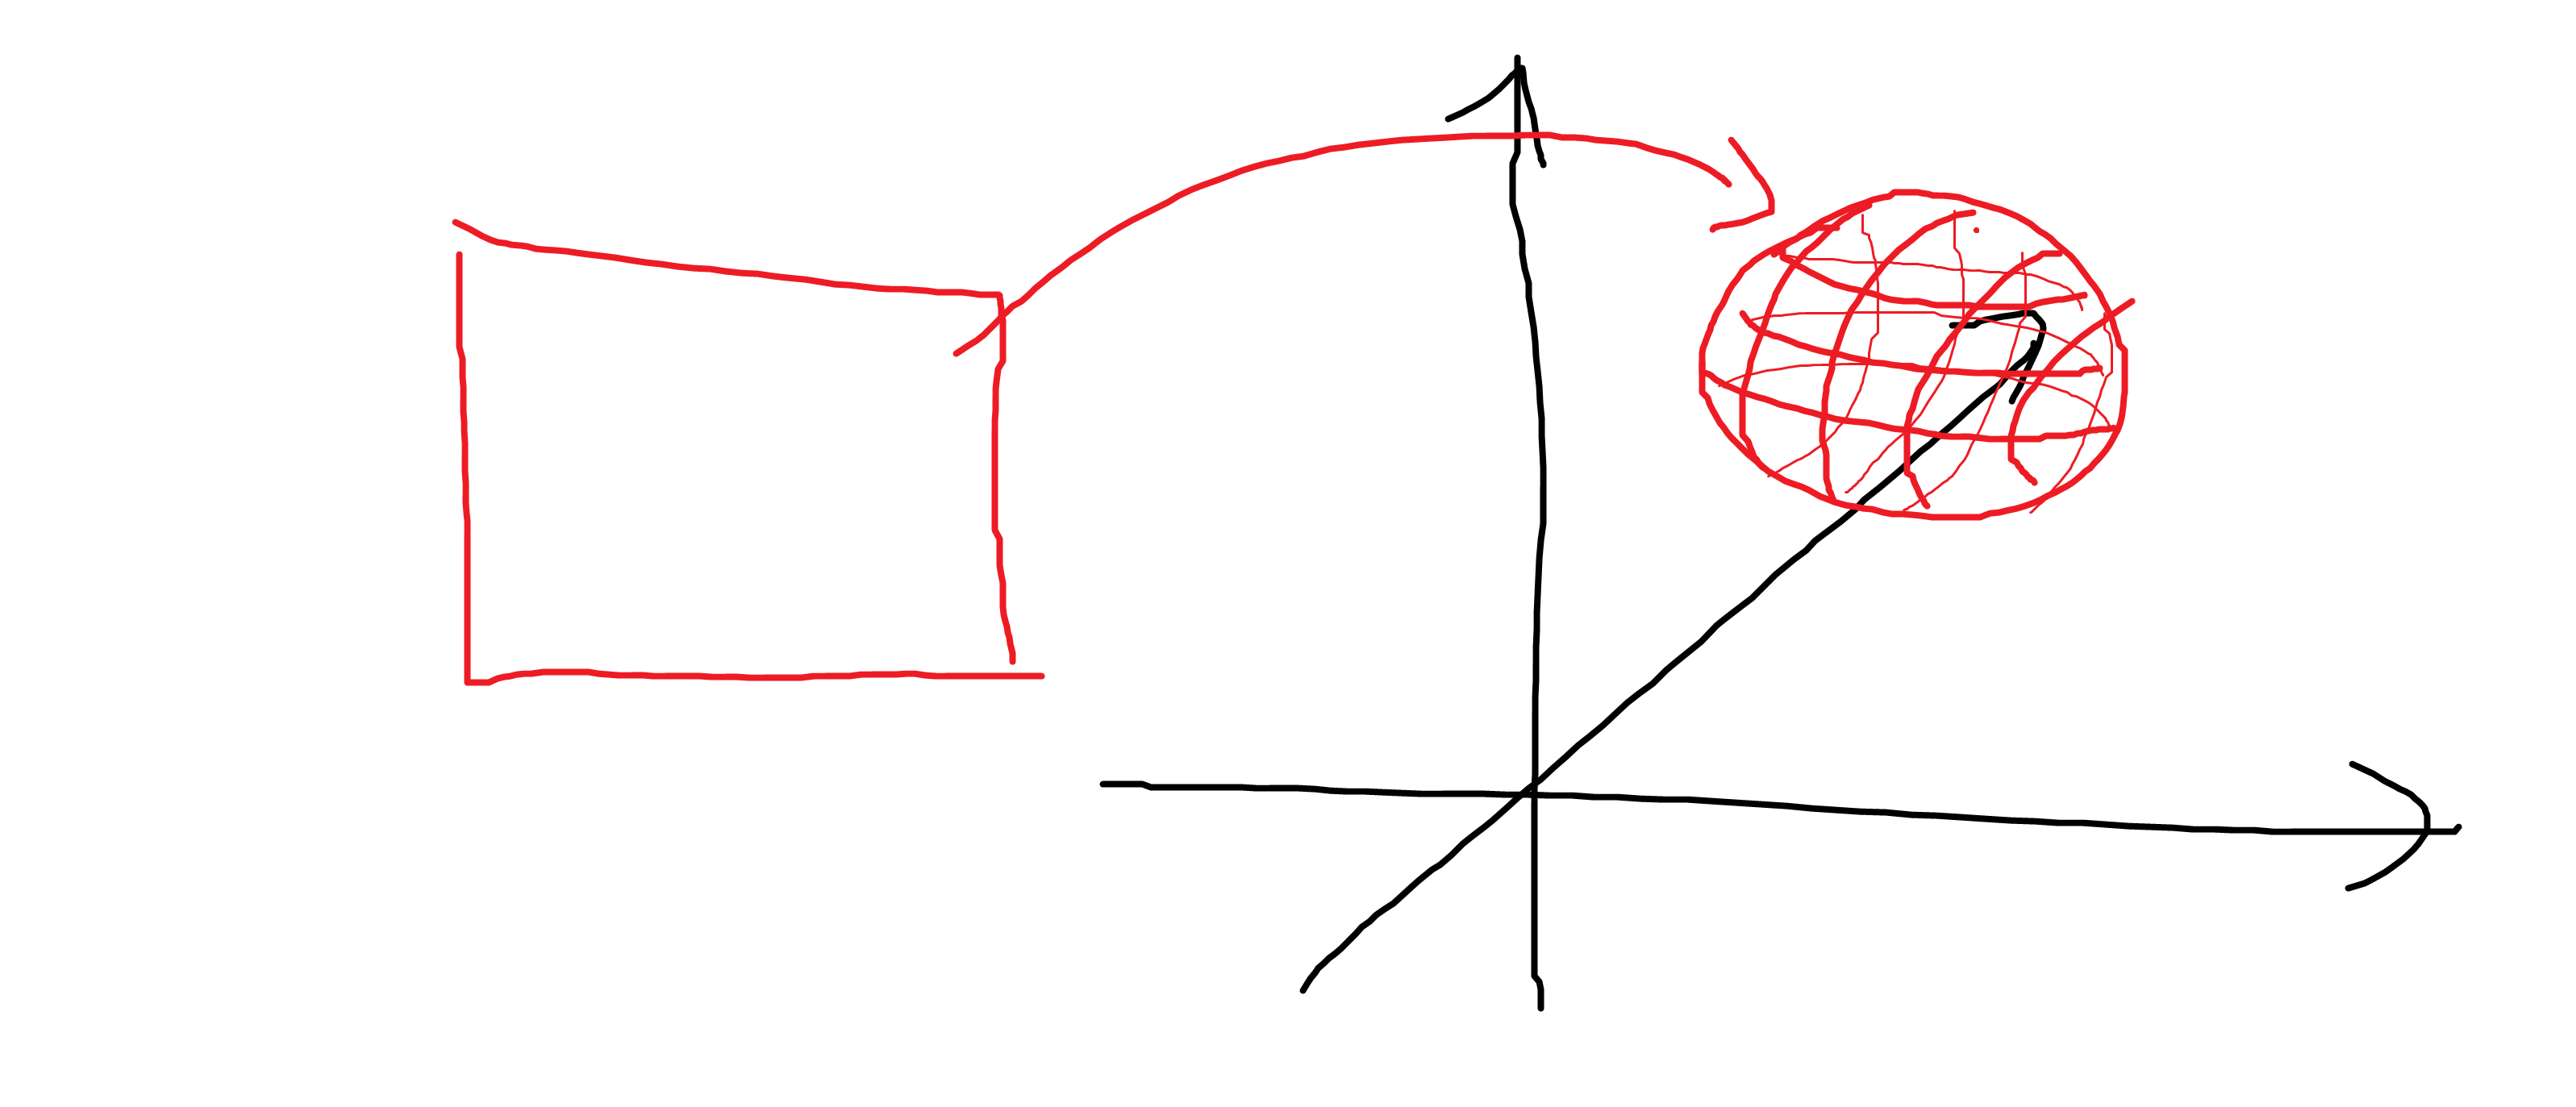
\includegraphics[height=3cm]{../2zh/kepek/29.png}
			\caption{Egy $\R^2\to\R^3$ leképezés}
		\end{figure}
		Legyen $h:=(x,y),\quad  a:=(1,2)$
		\[ f(a+h)-f(a)=f(x+1,y+2)-f(1,2)=\begin{bmatrix}
			(x+1)^3+(x+1)(y+2)\\
			x+1-(y+2)^2\\
			1+(y+2)
		\end{bmatrix}-\begin{bmatrix}
			3\\
			-3\\
			3
		\end{bmatrix}=\]
		\[=\begin{bmatrix}
			x^3+3x^2+3x+1+xy+2x+y+2-3\\
			x+1-y^2-4y-4+3\\
			y+3-3
		\end{bmatrix}=\begin{bmatrix}
		5x+y\\
		x-4y\\
		y
		\end{bmatrix}-\begin{bmatrix}
			x^3+3x^2+xy\\
			-y^2\\
			0
		\end{bmatrix} \]
		Legyen: $L(h):=L(x,y):=\begin{bmatrix}
		5x+y\\
		x-4y\\
		y
		\end{bmatrix}=\begin{bmatrix}
		5&1\\
		1&-4\\
		0&1
		\end{bmatrix}\cdot \begin{bmatrix}
		x\\
		y
		\end{bmatrix}$
		\[ 0\leq\lim_{(x,y)\to(0,0)}\frac{\norm{
				\begin{bmatrix}
					x^3+3x^2+xy\\
					-y^2\\
					0
				\end{bmatrix}
		}_{\R^3}}{\norm{(x,y)}_{\R^2}}=\lim_{(x,y)\to(0,0)}\frac{|x^2+3x^2+xy|+|-y^2|+|0|}{\norm{(x,y)}_\infty}\leq\]
		\[\leq \lim_{(x,y)\to(0,0)}\frac{|x|^3+3|x|^2+|x|\cdot|y|+|y|^2}{\norm{(x,y)}_\infty}\leq\lim_{(x,y)\to(0,0)}\frac{\norm{(x,y)}^3_\infty+5\norm{(x,y)}^2_\infty}{\norm{(x,y)}_\infty}=\]
		\[=\lim_{(x,y)\to(0,0)}(\norm{(x,y)}^2_\infty+5\norm{(x,y)}_\infty)=0^2+5\cdot0=0\quad \Rightarrow \]
		a def-beli $\lim=0\quad \Rightarrow
		\quad$
		\[ f\in D\{(1,2)\}\quad \text{és}\quad f'(1,2)=\begin{bmatrix}
			5&1\\
			1&-4\\
			0&1
		\end{bmatrix}\in\R^{3\times 2} \]
		\textit{Ellenőrzés:}
		Ha $f\in D\{(x,y)\}\quad \Rightarrow \quad (\forall (x,y)\in\R^2)$
		\[ f(x,y)=:\begin{bmatrix}
			f_1(x,y)\\
			f_2(x,y)\\
			f_3(x,y)
		\end{bmatrix}\quad \Rightarrow\quad f'(x,y)=\begin{bmatrix}
			\grad f_1(x,y)\\
			\grad f_2(x,y)\\
			\grad f_3(x,y)
		\end{bmatrix} =\begin{bmatrix}
			\partial_1 f_1(x,y)&\partial_2 f_1(x,y)\\
			\partial_1 f_2(x,y)&\partial_2 f_2(x,y)\\
			\partial_1 f_3(x,y)&\partial_2 f_3(x,y)
		\end{bmatrix}=\begin{bmatrix}
			3x^2+y&x\\
			1&-2y\\
			0&1
		\end{bmatrix} \]
		
		Enek a mátrixnak mind a 6 komponense folytonos fv (polinomok)$\quad \Rightarrow\quad f\in D(\R^2)$
	\end{task}
\end{document}